\section{Lemur总体架构分析}
Lemur是一种遵循lustre HSM架构的跨层冷热数据实现方案。lustre提供一套针对HSM相关的用户调用接口,由用户自定义实现满足业务需求的冷热数据迁移方案。Lemur与Lustre的关系图如下: 

\begin{figure}[!htb]
    \centering
    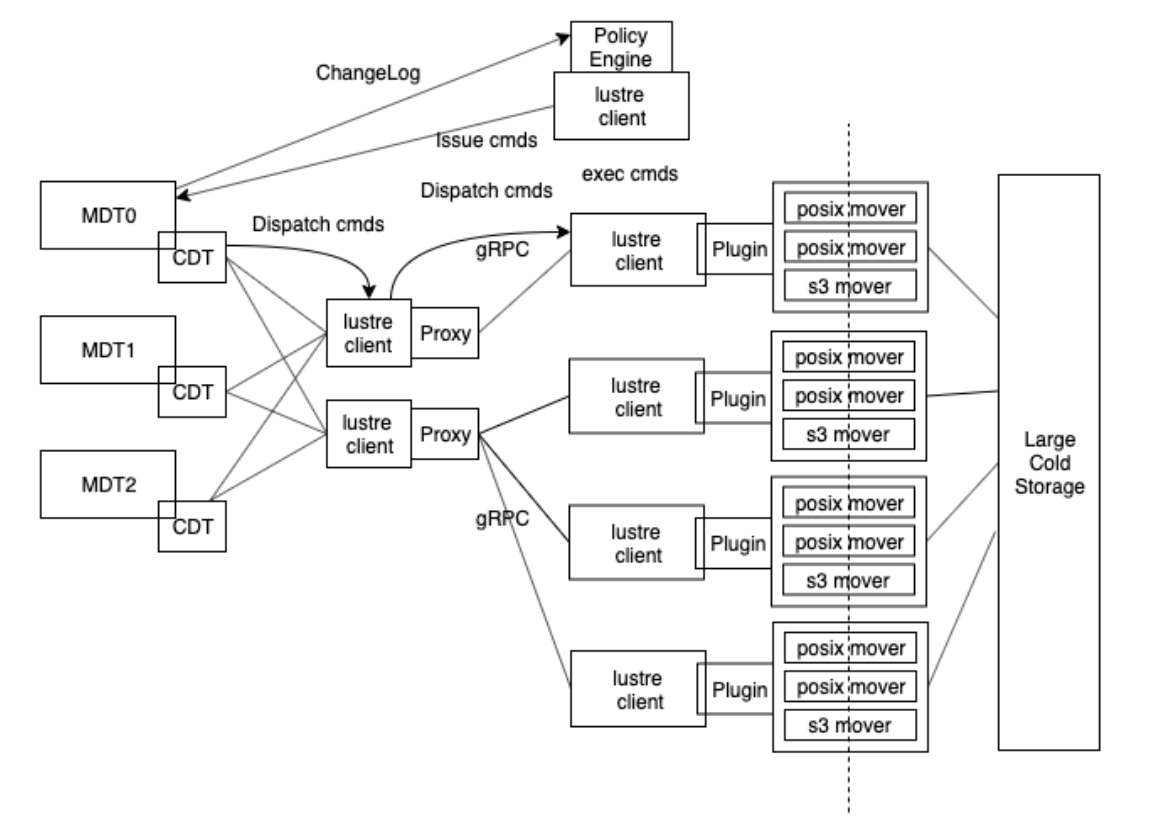
\includegraphics[width=\linewidth]{lemur.png}
    \caption{Lemur总体架构}\label{fig:region-image}
\end{figure}

上图中,对于每个MDT可以开启相应的HSM功能。开启lustre的HSM功能时,在会相应的MDT上启动一个Coordinator的守护进程,用于处理和派发HSM命令。Lemur在选定的lustre客户端上通过调用lustre的开发接口向所有开启HSM功能的MDT上注册一个或者多个Proxy。Proxy用于轮训来自MDT的HSM事件并接收其命令,之后将该命令按照一定的策略派发到相应的Copytool服务中。Copytool与Proxy通过gRPC连接,其所为gRPC的客户端存在,负责执行相应的HSM命令。 

每个MDT可以注册多个Proxy,MDT会按照一定的最佳选择策略将HSM命令派发到某个Proxy。每个Proxy可以连接多个Copytool,Proxy将HSM命令按照Archive ID与Copytool映射表,将HSM命令再次派发到对应的Copytool进行执行。每个Proxy最多可注册32个不同Archive ID的Copytool。Copytool执行具体的HSM命令时可以向Proxy返回其执行进度,以方便Proxy确认命令是否按时按需执行。 

每个Copytool同样运行在一个lustre客户端上,其包括Plugin和DataMover两个主要模块。Plugin是对DataMover集合的一种抽象的表示,每个DataMover作为PluginClient由Plugin模块进行管理,且DataMover可以按照pluginClient的接口由用户进行自定义。当前Lemur支持posix-to-posix的DataMover以及posix-to-s3的DataMover。顾名思义,不同的DataMover应对不同的HSM后端。posix DataMover可以将冷数据存储到支持posix接口的冷数据存储中,而s3 DataMover可以将冷数据存储到支持s3接口的冷数据存储中。 

除此之外,lustre的HSM架构中,还有一个PolicyEngine模块是必不可少的。PolicyEngine是运行在一个或者多个lustre客户端上的HSM策略服务,其通过lustre MDT导出的ChangeLog,收集存储在lustre中的元数据以及用户操作日志,并将这些日志存储到后端大数据分析平台中。这些数据会被用于分析当前lustre存储系统的状态和数据的分布及活动状况,通过用户定义HSM策略,执行相应的HSM命令。比如,可以将超过10天未被访问的某些类型的文件下沉到冷数据存储中;可以根据当前业务的需求按照某种数据预期策略提前将需要的数据预取到lustre中等操作。 
